% This is a LaTeX thesis template for Monash University.
% to be used with Rmarkdown
% This template was produced by Rob Hyndman
% Version: 6 September 2016

\documentclass{monashthesis}

%%%%%%%%%%%%%%%%%%%%%%%%%%%%%%%%%%%%%%%%%%%%%%%%%%%%%%%%%%%%%%%
% Add any LaTeX packages and other preamble here if required
%%%%%%%%%%%%%%%%%%%%%%%%%%%%%%%%%%%%%%%%%%%%%%%%%%%%%%%%%%%%%%%

\author{Dewi Lestari Amaliah}
\title{Thesis title}
\studentid{31251587}
\def\degreetitle{Master of Business Analytics}
% Add subject and keywords below
\hypersetup{
     %pdfsubject={The Subject},
     %pdfkeywords={Some Keywords},
     pdfauthor={Dewi Lestari Amaliah},
     pdftitle={Thesis title},
     pdfproducer={Bookdown with LaTeX}
}


\bibliography{thesisrefs}

\begin{document}

\pagenumbering{roman}

\titlepage

{\setstretch{1.2}\sf\tighttoc\doublespacing}

\clearpage\pagenumbering{arabic}\setcounter{page}{0}

\hypertarget{abstract}{%
\chapter*{Abstract}\label{abstract}}
\addcontentsline{toc}{chapter}{Abstract}

The abstract should outline the main approach and findings of the thesis and must not be more than 500 words.

\newpage

\hypertarget{acknowledgements}{%
\chapter*{Acknowledgements}\label{acknowledgements}}
\addcontentsline{toc}{chapter}{Acknowledgements}

I would like to thank my pet goldfish for \dots

\hypertarget{ch:intro}{%
\chapter{Introduction}\label{ch:intro}}

This is where you introduce the main ideas of your thesis, and an overview of the context and background.

Later chapters should be divided into coherent pieces describing your analysis. The final chapter should provide some concluding remarks, discussion, ideas for future research, and so on. Appendixes can contain additional material that don't fit into any chapters, but that you want to put on record. For example, additional tables, output, etc.

\hypertarget{rmarkdown}{%
\section{Rmarkdown}\label{rmarkdown}}

In this template, the rest of the chapter shows how to use Rmarkdown. The big advantage of using Rmarkdown is that it allows you to include your R code directly into your thesis, to ensure there are no errors in copying and pasting, and that everything is reproducible. It also helps you stay better organized.

For details on using \emph{R Markdown} see \url{http://rmarkdown.rstudio.com}.

\hypertarget{data}{%
\section{Data}\label{data}}

Included in this template is a file called \texttt{sales.csv}. This contains quarterly data on Sales and Advertising budget for a small company over the period 1981--2005. It also contains the GDP (gross domestic product) over the same period. All series have been adjusted for inflation. We can load in this data set using the following command:

\begin{Shaded}
\begin{Highlighting}[]
\NormalTok{sales <-}\StringTok{ }\KeywordTok{ts}\NormalTok{(}\KeywordTok{read.csv}\NormalTok{(}\StringTok{"data/sales.csv"}\NormalTok{)[,}\OperatorTok{-}\DecValTok{1}\NormalTok{], }\DataTypeTok{start=}\DecValTok{1981}\NormalTok{, }\DataTypeTok{frequency=}\DecValTok{4}\NormalTok{)}
\end{Highlighting}
\end{Shaded}

Any data you use in your thesis can go into the data directory. The data should be in exactly the format you obtained it. Do no editing or manipulation of the data outside of R. Any data munging should be scripted in R and form part of your thesis files (possibly hidden in the output).

\hypertarget{figures}{%
\section{Figures}\label{figures}}

Figure \ref{fig:deaths} shows time plots of the data we just loaded. Notice how figure captions and references work. Chunk names can be used as figure labels with \texttt{fig:} prefixed. Never manually type figure numbers, as they can change when you add or delete figures. This way, the figure numbering is always correct.

\begin{figure}
\centering
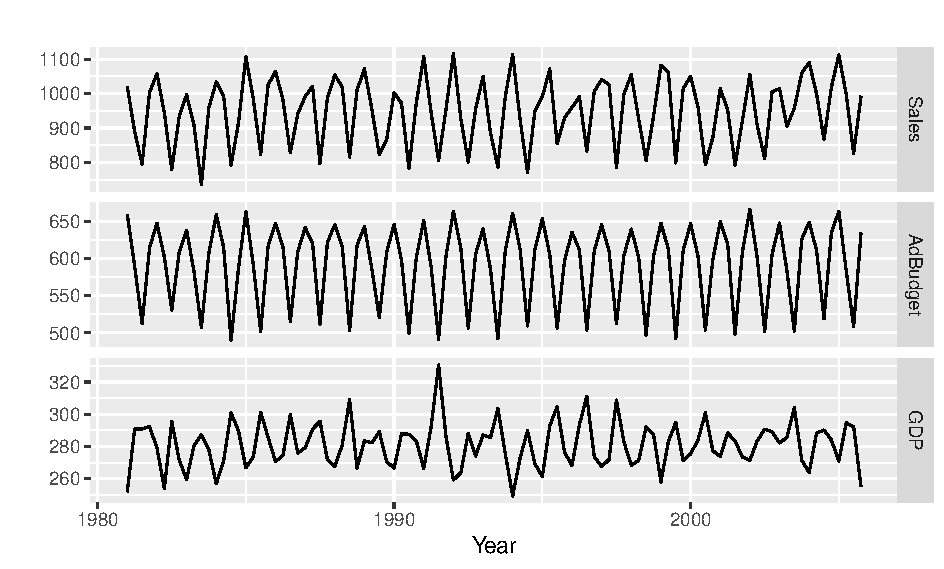
\includegraphics{thesis_files/figure-latex/deaths-1.pdf}
\caption{\label{fig:deaths}Quarterly sales, advertising and GDP data.}
\end{figure}

\hypertarget{results-from-analyses}{%
\section{Results from analyses}\label{results-from-analyses}}

We can fit a dynamic regression model to the sales data.

If \(y_t\) denotes the sales in quarter \(t\), \(x_t\) denotes the corresponding advertising budget and \(z_t\) denotes the GDP, then the resulting model is:
\begin{equation}
  y_t - y_{t-4} = \beta (x_t-x_{t-4}) + \gamma (z_t-z_{t-4}) + \theta_1 \varepsilon_{t-1} + \Theta_1 \varepsilon_{t-4} + \varepsilon_t
\end{equation}
where
\(\beta = 2.28\),
\(\gamma = 0.97\),
\(\theta_1 = NA\),
and
\(\Theta_1 = -0.90\).

\hypertarget{tables}{%
\section{Tables}\label{tables}}

Let's assume future advertising spend and GDP are at the current levels. Then forecasts for the next year are given in Table \ref{tab:salesforecasts}.

\begin{table}[ht]
\begin{center}
\begin{tabular}{lrrrr}
\toprule
Point Forecast & Lo 80 & Hi 80 & Lo 95 & Hi 95 \\
\midrule
1000.2 &  947.7 & 1052.7 & 919.9 & 1080.5 \\
1013.1 &  959.3 & 1066.8 & 930.9 & 1095.3 \\
1076.7 & 1022.9 & 1130.6 & 994.4 & 1159.0 \\
1003.5 &  949.7 & 1057.4 & 921.2 & 1085.8 \\
\bottomrule
\end{tabular}
\caption{Forecasts for the next year assuming Advertising budget and GDP are unchanged.}
\label{tab:salesforecasts}
\end{center}
\end{table}

Again, notice the use of labels and references to automatically generate table numbers. In this case, we need to generate the label ourselves.

The \texttt{knitLatex} package is useful for generating tables from R output. Other packages can do similar things including the \texttt{kable} function in \texttt{knitr} which is somewhat simpler but you have less control over the result. If you use \texttt{knitLatex} to generate tables, don't forget to include \texttt{results="asis"} in the chunk settings.

\hypertarget{sec:syslitrev}{%
\chapter{Systematic Literature Review}\label{sec:syslitrev}}

This study is performed using a systematic review method in which an attempt is made to collect empirical evidence explicitly and systematically using pre-specified eligibility criteria to answer a specific research question \autocite{cochrane}. Further, according to \textcite{brown_uni}, the key criteria of the systematic literature review are: \emph{``a clearly defined question with inclusion \& exclusion criteria; rigorous \& systematic search of the literature; critical appraisal of included studies; data extraction and management; analysis \& interpretation of results; and report for publication.''} Hence, to conform with these criteria, this study incorporates the Preferred Reporting Items for Systematic Reviews and Meta-Analysis (PRISMA)'s checklist and flow diagram. The following subsections discuss the steps conducted following those criteria.

\hypertarget{literature-identification}{%
\section{Literature Identification}\label{literature-identification}}

MRP is applied in various scientific fields, ranging from social and political science to public health. Therefore, to identify the literature, this study refers to research databases instead of field-specific journals. Those databases are JSTOR, EBSCO, and PubMed. The first two databases are chosen due to their broad range of field coverage, while the latter is chosen since MRP is sometimes also applied in the health and medical field. Choosing these databases also considers that heterogeneity of included studies is one of the important factors in a systematic literature review \autocite{SchweizerMarinL2017Apgt}.

Further, we identify the literature using the combination of several search terms. Mostly the search term includes the term ``multilevel regression,''post-stratification``,''poststratification``, and''multilevel model``. Our target literature is articles that are written in English. Regarding the time of publication, we exclude all of the publications before 1997 since the MRP method has not been developed in this period. Initially we included only the title/abstract when searching these databases. However, using this method limits the set of potential articles to only include those with the search term in the abstract/title. To rectify this, we also include a search with''all field" in the search criteria. Note that for EBSCO, we directly apply the search for all fields. The detailed literature identification is shown in Table \ref{tab:search-term}.

The total number of articles from this search criteria are 327. Next, we utilize the literature manager, EndNote X9, to manage these articles and to find duplicate articles. After removing those duplicate articles, we have 221 articles to be screened in the next stage.

\begin{landscape}\begin{table}

\caption{\label{tab:search-term}Detail of literature identification}
\centering
\resizebox{\linewidth}{!}{
\begin{tabular}[t]{l>{\raggedright\arraybackslash}p{15em}lllr}
\toprule
Database & Search Terms & Search Field & Inclusion & Exclusion & Number Returned\\
\midrule
JSTOR & (multilevel regression and poststratification) OR (“post-stratification”) & Abstract & Article, content I can access, English & anything before 1997 & 44\\
JSTOR & (("multilevel regression" AND ("post-stratification" OR Poststratification)) OR ("multilevel model" AND ("post-stratification" OR Poststratification))) & All field & Article, English & anything before 1997 & 142\\
EBSCO & "multilevel regression with post-stratification" OR "multilevel regression with poststratification" OR "multilevel regression and Poststratification" OR "multilevel regression and Post-stratification" & All field & Academic (Peer-Reviewed) Journals, English & anything before 1997 & 42\\
EBSCO & (multilevel regression AND post-stratification) OR (multilevel model AND post-stratification) OR (multilevel regression AND poststratification ) OR (multilevel model AND poststratification) & All field & Academic (Peer-Reviewed) Journals, English & anything before 1997 & 45\\
PubMed & "multilevel regression with post-stratification" OR "multilevel regression with poststratification" OR "multilevel regression and Poststratification" OR "multilevel regression and Post-stratification" & Title/Abstract & Article, English & anything before 1997 & 26\\
\addlinespace
PubMed & (multilevel regression AND post-stratification) OR (multilevel model AND post-stratification) OR (multilevel regression AND poststratification) OR (multilevel model AND poststratification) & All field & Article, English & anything before 1997 & 28\\
\bottomrule
\end{tabular}}
\end{table}
\end{landscape}

\hypertarget{screening-and-eligibility-criteria}{%
\section{Screening and Eligibility Criteria}\label{screening-and-eligibility-criteria}}

We screen all of the articles whether they fit the criteria to be included in the study or not. To screen efficiently, we use two stages. In the first stage DA and LK independently review all articles abstracts. Secondly DA reviews the full article to meet a second, more specific criteria.

\#\#\# Stage 1: Review of abstracts

In the first stage (abstract review)\ldots{}
- process
- criteria

with the following eligibility criteria:

\begin{enumerate}
\def\labelenumi{\arabic{enumi}.}
\tightlist
\item
  The abstract should mentions analysis of data or creation of simulation data.
\item
  The abstract should mentions use of MRP or multilevel models to make population estimates or the use of other regression models (BART, spatial, stacked, trees) to make population estimates.
\end{enumerate}

When the two reviewers (LK and DA) disagreed\ldots{}
- what happened
- how often did it happen

During the screening process, we find that 4 articles are apparently not research papers. In addition, we find that 104 articles that do not meet the criteria listed above. Therefore, we exclude them from the list.

\#\#\# Stage 2: Full manuscript review and coding

This leaves a remaing 113 articles for the second stage of the screening process. The aim of this stage is to get the list of the final articles that would be included in the study. We set the criteria of eligibility as follows:

\begin{enumerate}
\def\labelenumi{\arabic{enumi}.}
\tightlist
\item
  It should apply MRP as its method.
\item
  It should contain at least one plot relate to MRP findings.
\end{enumerate}

Dewi, I think this is confusing steps 1 and 2 from the two stages. Better to seperate it under the headings I've suggested, I think!

From the first sub-stage alone (i.e., abstract screening) we found that 61 articles fulfill the first criteria, which is using MRP as its method. Hence, we read the full articles for the remaining 52 articles. From this, we exclude 42 articles. Most of these articles are excluded because they do not meet Criteria 1, which is not using MRP as its method. These articles are captured in the first sub-stage mainly because they mention the search term (i.e., ``multilevel model'' or ``post-stratification'') in them. Many of them only use a common stratification weighting. Also, some articles using another method, but they mention MRP in their literature review as an alternative method to do the analysis. Other articles are excluded because they do not meet Criteria 2, which is does not convey their MRP result in a single plot.

Finally, we have 71 articles to be reviewed in the next stage. Figure \ref{fig:prisma-flowchart} displays the PRISMA flow chart of this study. This figure is generated using \textbf{\texttt{PRISMA2020}} \autocite{prisma2020}.

\hypertarget{data-extraction-and-analysis}{%
\section{Data Extraction and Analysis}\label{data-extraction-and-analysis}}

We focus the data extraction to the MRP-related plot. We manually create a metadata for each plot (included in supplementary material of this study). The reasons we create a metadata for these plots are to ensure the reproducibility of the analysis and to maintain the transparency of the systematic literature review process.

LK: We also collect this data to allow us to analyse the current reporting practices with MRP

To build a metadata we classify the plot into two types, i.e., communication (coded to 0) and diagnostic plot (coded to 1). For diagnostic plots, we examine whether the plots compare MRP with other estimates, which are:

\begin{enumerate}
\def\labelenumi{\arabic{enumi}.}
\tightlist
\item
  raw (direct estimates or direct disaggregation);
\item
  truth;
\item
  weight estimation;
\item
  estimates of other MRP models, for example, the paper build several MRP models from various simulation scenarios or using different covariates;
\item
  estimates from another study/survey;
\item
  estimates from another method, for example comparing MRP with Bayesian Additive Tress with Post-Stratification.
\end{enumerate}

Plot that show a comparison of MRP with each of the above list would be coded to 1, otherwise coded to 0.
The diagnostic plot could also display the performance of MRP using several performance criteria, as follows:

\begin{enumerate}
\def\labelenumi{\arabic{enumi}.}
\tightlist
\item
  Bias;
\item
  Mean Absolute Error (MAE);
\item
  Mean Square Error (MSE)/ Relative Mean Square Error (RMSE);
\item
  Standard Error (SE);
\item
  Correlation.
\end{enumerate}

Just like the comparison, the MRP-related plot would be reviewed whether it is contains each of those performance criteria (coded 1) or not (coded 0).

We also review other features of the plot using the grammar in \textbf{\texttt{ggplot2}} \autocite{ggplot2}. We examine the facet, plot type, what is put in the x, y-axis, color, and shape. Besides, the metadata also contains the paper's author/s, paper's year, paper's title, and plot's figure number.

LK: Also note why we chose to note the grammar and what we hoped to learn from it.

After the extraction, we analyze the data using graphical visualization with \textbf{\texttt{ggplot2}}. The result will be discussed in the next section.

\begin{figure}
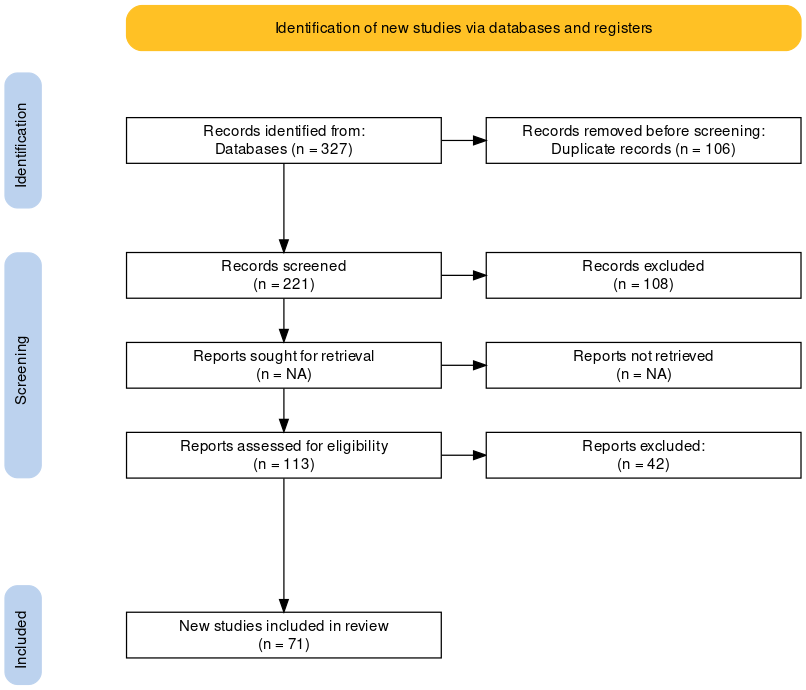
\includegraphics[width=0.9\linewidth]{figures/prisma_fc} \caption{PRISMA folow chart of this systematic literature review.}\label{fig:prisma-flowchart}
\end{figure}

\appendix

\hypertarget{additional-stuff}{%
\chapter{Additional stuff}\label{additional-stuff}}

You might put some computer output here, or maybe additional tables.

Note that line 5 must appear before your first appendix. But other appendices can just start like any other chapter.

\printbibliography[heading=bibintoc]



\end{document}
